\documentclass{report}
\usepackage[toc,section=section]{glossaries}
\usepackage{graphicx}
\usepackage{rotating}
\usepackage{pdflscape}
\usepackage{float}
\usepackage{listings}


% Title Page
\title{%
	EDB: Debugger for Ethereum's Programming Languages \\
	\medskip
	\large Report \#3: Requirements Specification \\
	\large Advised by Dr. Jackowitz	\\
	\large University of Scranton}
\author{Andrew Plaza}

\newglossaryentry{blockchain}{name=Blockchain,description={A growing list of records stored using some datastructure (usually a variation of a tree) and linked through cryptography}}
\newglossaryentry{dapp}{name=Decentralized Application, description={An application made specifically for Ethereum, which runs on the Ethereum Main Network}}
\newglossaryentry{solidity}{name=Solidity, description={A Javascript-like Programming Language that compiles down to EVM Bytecode}}
\newglossaryentry{vyper}{name=Vyper, description={A Python-like programming language that compiles down to EVM Bytecode}}
\newglossaryentry{LLL}{name=LLL, description={A Lisp-like programming language that compiles down to EVM Bytecode}}
\newglossaryentry{evm}{name=Ethereum Virtual Machine, description={A stack-based virtual machine created specifically for executing Ethereum Bytecode. It is part of the main ethereum protocol and is present in any Ethereum Node}}
\newglossaryentry{vscode}{name=Visual Studio Code, description={A popular code editor created by Microsoft}}
\newglossaryentry{rpc}{name=RPC, description={'Remote Procedure Call' is a protocol specification that outlines how a server should react to data sent to it}}
\newglossaryentry{parity}{name=Parity, description={An Ethereum Node Client written in Rust. Many of EDB's libraries rely on libraries that were created by the Parity team}}
\newglossaryentry{geth}{name=Geth, description={An Ethereum Node Client written in the Go programming language}}
\newglossaryentry{ethereumj}{name=EthereumJ, description={An Ethereum Node Client written in the Java programming language}}
\newglossaryentry{ethereumjs}{name=EthereumJS, description={An Ethereum Node Client written in the Javascript programming language, using the NodeJS runtime}}
\newglossaryentry{cppethereum}{name=cpp-ethereum, description={An Ethereum Node Client written in the C++ programming language}}
\newglossaryentry{rust}{name=Rust,description={a systems programming language with performance comparable to C/C++, but which prevents segfaults, and guarantees thread safety.}}
\newglossaryentry{eip}{name=Ethereum Improvement Proposal,description={Community-reviewed proposals anyone may submit to the Ethereum Foundation for review and discussion. If they are merged, they become part of the official Ethereum Protocol}}
\newglossaryentry{gplv3}{name=GPLv3 GNU General Public License, description={The GNU General Public License is a widely used free software license, which guarantees end users the freedom to run, study, share and modify the software }}


\makeglossaries
\begin{document}
\maketitle
\tableofcontents
\newpage

\section{Introduction}
Ethereum and \Gls{blockchain} technology have the potential to produce an entirely new era of technology more disruptive and transformative than the Internet. This project works with the core of what Ethereum is, providing developers who work with the core Ethereum \gls{blockchain} a more intuitive experience. Ultimately, this means faster development and the proliferation of \glspl{dapp}

Developers hoping to write new \glspl{dapp} in Ethereum-specific programming languages such as \gls{solidity}, \gls{vyper} and \gls{LLL} will be able to meticulously examine the state of their code at different points of execution taken by the \gls{evm}. This includes being able to see the internal \gls{evm} stack, and memory. In addition, the developer will be able to control the VM's execution; stopping it at a line in their code, continuing from a specific position, or stepping backward. Lastly, the developer may choose to inspect variables and their values that are in use in their code. All these functions will be available to be used with any Ethereum Node the developer may use for development. Additionally, The un-opinionated design of the libraries is such that it may be adapted to multiple different developer environments.

\section{System Model}
(figure on next page)
\begin{landscape}
	\begin{figure}
	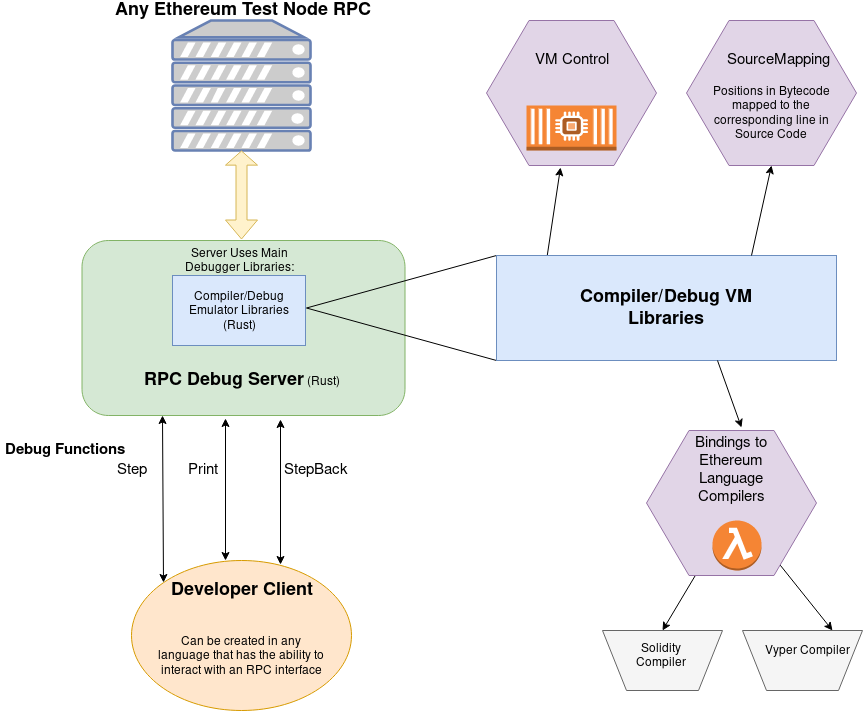
\includegraphics[height=\textheight]{SystemModel.png}
	\end{figure}
\end{landscape}
\newpage

\section{Functional Requirements}
The developer will be able to conduct all debug functions from a client application. There may be multiple possible client applications, but they will all provide the same debug functions. Differences exist only in how they are presented to the user. For example, \gls{vscode} may have a button representing 'step forward', while a Command-Line Client would instead take the command 'step'.

A client will be able to enter into a debug session for a specific source file. The client will then provide some functions available to the user in order to debug the source file that has been selected. The user will see this basic functionality at their disposal:
\begin{itemize}
	\item \textbf{help | ?}: Display a help message containing all available commands
	\item \textbf{version}: Display the current version of `edb` that is being used
	\item \textbf{step}: step forward to the next source-line in execution
	\item \textbf{stepback}: step back one source-line in execution
	\item \textbf{print}: print stack, memory, or variables in the program
	\item \textbf{printline}: print the current line in the source code that execution is at
	\item \textbf{printlines}: print a number of lines relative to the current line code execution is at in source code (two subcommands are available, each which accept a number argument. This would be used as such: `printlines previous 10` to print the 10 previous lines).
	\begin{itemize}
		\item \textbf{previous}: print lines previous to current line
		\item \textbf{next}: print lines after the current line
	\end{itemize}
	\item \textbf{exit | quit}: exit the client
	\item \textbf{breakpoint}: set a breakpoint at a line number in the source code where execution will stop
	\item \textbf{restart}: restart execution entirely
	\item \textbf{run}: run a function in the source code (accepts arguments according to function parameters)
	\item \textbf{continue}: Continue execution to the next breakpoint
	\item \textbf{previous}: Take execution back to the previous breakpoint
	\item \textbf{stepinto}: Step into a function (if the current line contains a function call)
\end{itemize}

\section{Non-Functional Requirements}
In order to use EDB, the user will need to set up a local Ethereum Node that exposes an \gls{rpc} interface and may be used in 'testnet' mode. Many variants of these applications exist, and the user is not constrained to a particular implementation. For example the user may choose between \Gls{parity}, \Gls{geth}, \Gls{cppethereum}, \Gls{ethereumj} or \Gls{ethereumjs}. A node running in 'testnet mode' is not connected to the Ethereum Mainnet, and as such does not have the same storage requirements or require an internet connection. The user will need at least 1GB of storage for the test node.

In addition to this, the user is required to run at least Linux, MacOSX, or Windows. Only these operating systems are supported. Embedded versions of these operating systems are not supported. Depending on the language the user is planning to debug, they will need to posses the official compiler available for their system. For instance, debugging \Gls{solidity} code requires that the 'solc' compiler is installed.

Code design and layout will follow official \Gls{rust} Language guidelines\footnote{Rust Style Guidelines \textit{https://github.com/rust-lang-nursery/fmt-rfcs/blob/master/guide/guide.md}}. In addition, Every public method, struct, and function in the resulting libraries from this project will be doc-commented to allow for document-generation. The project itself and all of it's libraries will be licensed under the \gls{gplv3}.


\section{User Interface Specification}

To initiate a debug session, the user will type the \lstinline[language=bash]{`edb`} command into their terminal-emulator of choice. The `edb` command accepts one argument when debugging: the path to the source file to debug. For example, a user may type \lstinline[language=bash]{edb ./my_program.sol}. The user is then greeted with the edb welcome screen and a command prompt. Typing in a command which is not recognized by the client will result in an error message denoting that the client does not recognize the command, and that the user may type the command 'help' or '?' to display a list of available commands. At any point in time, the user may use the 'exit' or 'quit' commands to close `edb`.

A typical debug session consists of a user first using the `breakpoint` command to set breakpoints at locations in the source code. The user can then start program execution with the 'run' command. Since Ethereum does not have the concept of a 'main' function, the 'run' command accepts arguments pertaining to the function and parameters the user intends to run. EDB will execute the users program up until the first breakpoint it hits. At that point, the user may choose to 'step' to the next line of code, 'stepback' to the previous line, 'print' the current values of variables, the stack, and memory, or 'restart' execution entirely. In addition, the user has the option of printing the current line, or an amount of next or previous lines of source code with the 'printlines' command. Finally, the user may use the 'continue' command to continue execution to the next breakpoint they set, or the 'previous' command to go back to the last breakpoint they set.

\section{System Evolution}

The fundamentals of the project is written in \Gls{rust}. While this is a slightly risky choice since \Gls{rust} is a relatively new language, it has a promising community and is backed by Mozilla. \Gls{rust} is used in a few well-known production applications; mainly the Firefox web-browser. Therefore, support for \Gls{rust} will be available for the foreseeable future. Since the language is still new, however, maintenance will be needed for language constructs which are changing or being added, as well as refactoring done when older code is phased out and no longer idiomatic.

The next part of my project that will need to be maintained is the Ethereum \gls{evm} and compilers. Ethereum is still a new application, so it's languages and protocols are never set-in-stone. Part of the maintenance of EDB will include keeping up-to-date with \glspl{eip} and implementing them if any are accepted and effect the execution of \glspl{dapp}. The libraries being used by EDB are open-source, and created by Parity Technologies. \Gls{parity} is currently one of the main and most popular Ethereum Node Clients, so the maintenance of the libraries may be ensured for as long as \Gls{parity} and Ethereum exist. It is, however, problematic if Parity Technologies happens to stop development of these libraries. In this worst-case scenario, since the libraries are under the \gls{gplv3}, the code may be forked and maintained as part of the debugger.

\printglossary[title={Glossary | Index}]

\end{document}
